\documentclass[sisc-eikonal.tex]{subfiles}

\begin{document}

\section{Numerical Results}\label{sec:numerical-results} In this
section, we collect our numerical tests. We first test our factored
method on several different slowness functions with available exact
solutions for point source data. We also test our method on a linear
speed function (reciprocal of slowness) which has been shown to be
amenable to local factoring. Finally, we present some statistics on
the number of different types of updates performed by
\cref{alg:bottom-up,alg:top-down} to give a more precise understanding
of the types of updates that make up the majority of each method's
runtime.

\subsection[Single point source]{Nonsymmetric slowness functions with
  a single point source}\label{ssec:point-source-problems}

\begin{table}
  \centering
  \begin{tabular}{cccc}
    Name & $u(x)$ & $s(x)$ \\
    \midrule
    \texttt{s0} & $r$ & $1$ \\
    \texttt{s1} & $\cos(r) + r - 1$ & $1 - \sin(r)$ \\
    \texttt{s2} & $r^2/2$ & $r$ \\
    \texttt{s3} & $S^\top A S$ & $\alpha\norm{\operatorname{diag}(C){(A + A^\top)}S}$ \\
    \texttt{s4} & $\tfrac{1}{2} x^\top A^{1/2} x$, where $A$ is symmetric positive definite & $\norm{x}_A = \sqrt{x^\top A x}$
  \end{tabular}
  \caption{Slowness functions used in point source tests. For these
    definitions, we assume that $x \in \Omega = [-1, 1]^n$, where
    $n = 2, 3$. Each definition is for $n = 2$ and $n = 3$. We also
    define $r = \norm{x}$, $S = (\sin(\alpha x_i))_{i=1}^n$, and
    $C = (\cos(\alpha x_i))_{i=1}^n$. \hl{\textbf{TODO}}:
    \emph{\texttt{s2}--\texttt{s4} don't have a singularity like
        \texttt{s0} and \texttt{s1} do and don't need to be factored. We
        could make these better examples by adding $r$ to \texttt{s2}
        and replacing \texttt{s3} and \texttt{s4} with their square
        roots.}}\label{table:slowness-functions}
\end{table}

Using \cref{eq:eikonal} directly, a simple recipe to create pairs of
slowness functions $s$ and solutions $u$ is to prescribe a solution
$u$ and compute $s(x) = \norm{\nabla u(x)}_2$. See
\cref{table:slowness-functions} for slowness function definitions. In
2D, the matrices we use for \texttt{s3} and \texttt{s4} are:
\begin{equation}
  A_{\texttt{s3}} = \begin{bmatrix}
    2 & 1 \\
    1 & \nicefrac{1}{2}
  \end{bmatrix}, \qquad A^{1/2}_{\texttt{s4}} = \begin{bmatrix}
    \nicefrac{2}{3} & \nicefrac{-1}{2} \\
    \nicefrac{-1}{2} & 1
  \end{bmatrix},
\end{equation}
and in 3D:
\begin{equation}
  A_{\texttt{s3}} = \begin{bmatrix}
    1 & \nicefrac{1}{4} & \nicefrac{1}{8} \\
    \nicefrac{1}{4} & 1 & \nicefrac{1}{4} \\
    \nicefrac{1}{8} & \nicefrac{1}{4} & 1
  \end{bmatrix} = A_{\texttt{s4}}^{1/2}
\end{equation}
Plots collecting our numerical results are contained in
\cref{sec:point-source-plots}. For the algorithms listed in
\cref{ssec:specific-algorithms}, we include plots of relative $\ell_2$
and $\ell_\infty$ error plotted versus problem size and time.

\subsection{A linear speed function}\label{ssec:slotnick}

\begin{figure}[t]
  \centering
  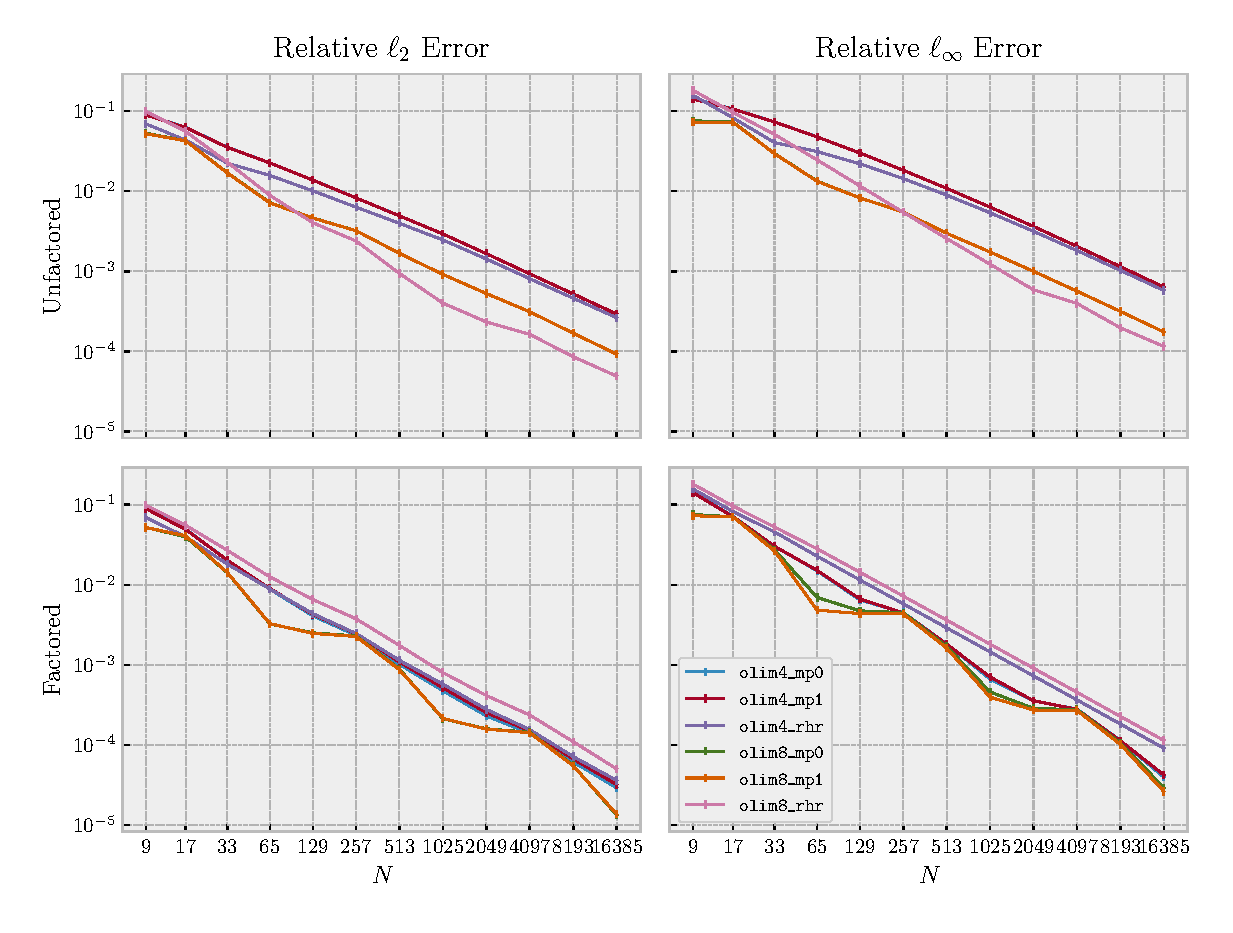
\includegraphics[width=\linewidth]{qv_plots_2d.eps}
  \caption{Comparing factoring using a linear speed function: relative
    error plots in 2D for \cref{ssec:slotnick}. For these plots,
    $\Omega = [0, 1]^2$, and $N$ is the number of grid points that
    each side of the square $\Omega$ is discretized into. There are
    two point sources at $(0, 0)$ and $(0.8, 0)$. The disks of radius
    $\rfac = 0.1$ around each point are factored. We note that in this
    example, the errors due to the linear interpolation and the use of
    the \texttt{rhr} quadrature rule partially compensate each
    other. \hl{\textbf{TODO}}: \emph{extend these plots to a larger
      size on the cluster before submitting.}}\label{fig:qv-2d}
\end{figure}

We consider a problem that has an analytical ray tracing solution and
is used as a test problem elsewhere for solvers for the factored
eikonal
equation~\cite{slotnick1959lessons,fomel2009fast,qi2018corner}. For a
single point source at $x_i$ and a vector $v$, we define:
\begin{equation}
  \label{eq:slotnick-single-source}
  \frac{1}{s_i(x)} = \frac{1}{s_i} + v^\top {(x - x_i)},
\end{equation}
hence $s_i(x_i) = s_i$. The analytic solution to \cref{eq:eikonal} for a
single source and slowness function given by
\cref{eq:slotnick-single-source} is:
\begin{equation}
  \label{eq:slotnick-single-source-solution}
  u_i(x) = \frac{1}{\norm{v}} \cosh^{-1} \parens{1 + \frac{s_i}{2} s(x) \norm{v}^2 \norm{x - x_i}^2}.
\end{equation}
If we shift the point source from $x_i$ to another location $x_j$, we
find:
\begin{equation}
  \label{eq:slotnick-slowness-shift}
  \frac{1}{s_i(x)} = \frac{1}{s_i} + v^\top {(x - x_j + x_j - x_i)} = \frac{1}{s_i} + v^\top {(x_j - x_i)} + v^\top {(x - x_j)} = \frac{1}{s_i(x_j)} + v^\top {(x - x_j)}.
\end{equation}
Defining $s_j = s_i(x_j)$ and $s_j(x)$ from:
\begin{equation}
  \frac{1}{s_j(x)} = \frac{1}{s_j} + v^\top {(x - x_j)},
\end{equation}
we can see that $s_j(x_i) = s_i(x_j)$, that shifting the point source
from $x_i$ to $x_j$ is equivalent to changing the parameter $s_i$ to
$s_j$, and that $u_j(x)$ is defined analogously to
\cref{eq:slotnick-single-source-solution}. The solution for multiple
point sources $\set{x_i}$ is then given
by~\cite{fomel2009fast,qi2018corner}:
\begin{equation}
  u(x) = \min_i u_i(x).
\end{equation}

\begin{figure}[t]
  \centering
  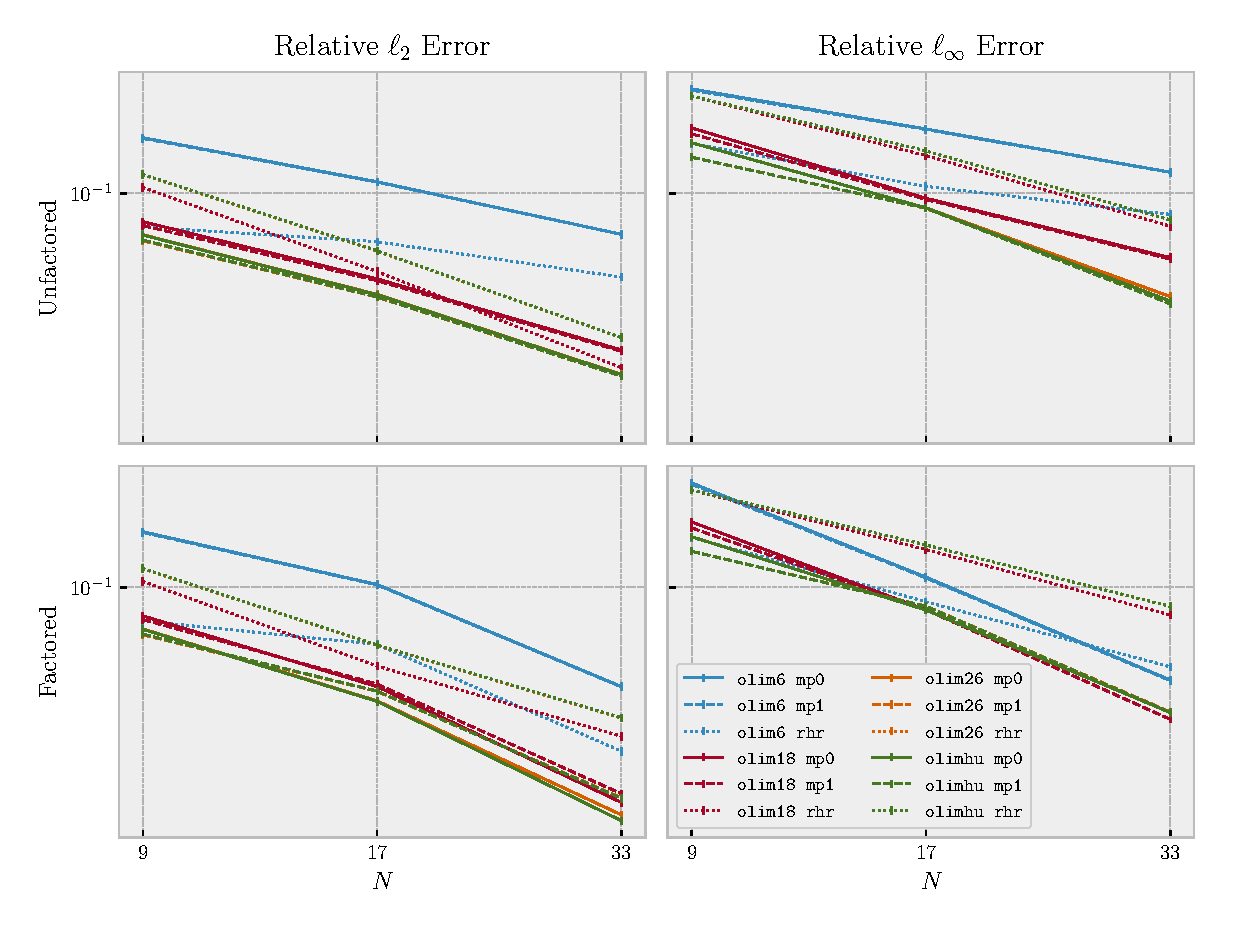
\includegraphics[width=\linewidth]{qv_plots_3d.eps}
  \caption{Comparing factoring using a linear speed function: relative
    error plots in 3D for \cref{ssec:slotnick}. For these plots,
    $\Omega = [0, 1]^3$, and $N$ is the number of grid points that
    each side of the square $\Omega$ is discretized into. There are
    two point sources at $(0, 0, 0)$ and $(0.8, 0, 0)$. The disks of
    radius $\rfac = 0.1$ around each point are factored. Compared to
    the example in \cref{fig:qv-2d}, we simply add a third dimension
    and keep the rest of the problem the same. The same comments
    regarding the quadrature rule \texttt{rhr} apply
    here. \hl{\textbf{TODO}}: \emph{extend these plots to a larger
      size on the cluster before submitting.}}\label{fig:qv-3d}
\end{figure}

We compare relative $\ell_2$ and $\ell_\infty$ errors in for each of
our OLIMs in 2D and 3D for this slowness function. See
\cref{fig:qv-2d,fig:qv-3d}.

\subsection{Comparison of hierarchical algorithms}\label{ssec:alg-comparison}

\Cref{alg:bottom-up,alg:top-down} can be compared in terms of the
number of updates of different degree that they
perform. In~\cref{tab:stats}, for our usual single point source
problem on $\Omega = [-1, 1]^3$, discretized into a grid with $n^3$
points, where $n = 5, 9, \hdots, 129$, we run \texttt{olim6},
\texttt{olim18}, \texttt{olim26}, and \texttt{olimhu}, using the
\texttt{rhr} quadrature rule for each (the choice of quadrature rule
has no bearing on this experiment). For each algorithm, we compute the
average number of times each node is visited, and the average number
of line, triangle, and tetrahedron updates that are performed. For the
triangle and tetrahedron updates, we count the number of updates that
are ``nondegenerate''---i.e, which have an interior point solution and
contribute information to the solution. From these statistics, we can
see numerically that the total number of updates of each type is
$O(N)$, which matches our expectations. Further, we can see that a
reasonably small number of updates is performed.

\begin{table}
  \centering
  \begin{tabular}{c|r|r|r|r|r}
& $N$ & Avg. Visits & $d = 0$ & $d = 1$ & $d = 2$ \\
\midrule
\multirow{6}{*}{\texttt{olim18\_rhr}} & 5 & 6.2400 & 1.0000 & 1.2481 & 0.1916 \\
& 9 & 7.4074 & 1.0000 & 1.2526 & 0.2738 \\
& 17 & 8.1384 & 1.0000 & 1.2426 & 0.3187 \\
& 33 & 8.5510 & 1.0000 & 1.2338 & 0.3477 \\
& 65 & 8.7707 & 1.0000 & 1.2284 & 0.3624 \\
& 129 & 8.8841 & 1.0000 & 1.2254 & 0.3702 \\
\midrule
\multirow{6}{*}{\texttt{olim26\_rhr}} & 5 & 8.2880 & 1.0000 & 0.5453 & 0.0962 \\
& 9 & 10.2167 & 1.0000 & 0.5202 & 0.1843 \\
& 17 & 11.4732 & 1.0000 & 0.4930 & 0.2382 \\
& 33 & 12.1982 & 1.0000 & 0.4774 & 0.2638 \\
& 65 & 12.5889 & 1.0000 & 0.4696 & 0.2762 \\
& 129 & 12.7918 & 1.0000 & 0.4656 & 0.2822 \\
\midrule
\multirow{6}{*}{\texttt{olimhu\_rhr}} & 5 & 8.2880 & 1.0000 & 1.1886 & 0.6547 \\
& 9 & 10.2167 & 1.0000 & 1.3074 & 0.8064 \\
& 17 & 11.4732 & 1.0000 & 1.3629 & 0.8626 \\
& 33 & 12.1982 & 1.0000 & 1.3890 & 0.8773 \\
& 65 & 12.5889 & 1.0000 & 1.4022 & 0.9062 \\
& 129 & 12.7918 & 1.0000 & 1.4092 & 0.9099 \\
\midrule
\multirow{6}{*}{\texttt{olim6\_rhr}} & 5 & 2.4000 & 1.0000 & 1.0753 & 0.1720 \\
& 9 & 2.6667 & 1.0000 & 1.2015 & 0.2344 \\
& 17 & 2.8235 & 1.0000 & 1.2682 & 0.2780 \\
& 33 & 2.9091 & 1.0000 & 1.3013 & 0.3039 \\
& 65 & 2.9538 & 1.0000 & 1.3175 & 0.3182 \\
& 129 & 2.9767 & 1.0000 & 1.3255 & 0.3256 \\
\midrule
\end{tabular}

  \caption{Table of update statistics
    for~\cref{ssec:alg-comparison}. All numbers are averages per grid
    point. Above, ``nondeg.'' is ``nondegenerate''. As $N$ increases,
    the average number of updates of each type per grid point
    approaches a constant. It's clear that only $O(N)$ updates of each
    type should be performed total---this gives numerical evidence
    that the constant in this $O(N)$ is small and a minimal number of
    updates of each type are evaluated.}
  \label{tab:stats}
\end{table}

\end{document}

%%% Local Variables:
%%% mode: latex
%%% TeX-master: "sisc-eikonal.tex"
%%% End:
